% Chapter 1

\chapter{The theory of lepton anomalous magnetic moments} % Main chapter title

\label{Chapter1} % For referencing the chapter elsewhere, use \ref{Chapter1} 

%----------------------------------------------------------------------------------------

% Define some commands to keep the formatting separated from the content 
\newcommand{\keyword}[1]{\textbf{#1}}
\newcommand{\tabhead}[1]{\textbf{#1}}
\newcommand{\code}[1]{\texttt{#1}}
\newcommand{\file}[1]{\texttt{\bfseries#1}}
\newcommand{\option}[1]{\texttt{\itshape#1}}

%----------------------------------------------------------------------------------------
\section{Lepton magnetic dipole moments}
 
In Particle Physics, the study of the anomalous magnetic moment of the muon is particularly fascinating due to the wide range of Standard Model (SM) physics it is sensitive to and the precision with which it can be measured both experimentally and predicted theoretically. It also provides a sensitive probe into Beyond Standard Model (BSM) physics. 
 
The magnetic dipole moment relates the torque experienced by a charged particle to the external magnetic field. The torque acts perpendicular to both the magnetic dipole moment and the magnetic field and causes the magnetic dipole moment to precess about the direction of the magnetic field at the so called Larmor frequency. An example being a compass needle aligning itself with the Earth’s magnetic field. 

In quantum mechanics charged particles with a non-zero spin have an intrinsic magnetic dipole moment $\mu$ arising from the spin, even when at rest \cite{Reference1}. 
The magnetic dipole moment for a spin-$\frac{1}{2}$ charged particle is given by:

\begin{equation}
\vec{\mu} = g\frac{Qe}{2m}\vec{s},
\end{equation}
where $g$ is the gyromagnetic ratio, $Q$ is the sign of the charge, $e$ is the charge of the particle, m is its mass and $\vec{s}$ is the spin of the particle. 
The gyromagnetic ratio, also known as the $g$-factor, is the dimensionless proportionality constant relating the angular momentum and the intrinsic magnetic moment.

After the discovery of spin, Dirac predicted that the gyromagnetic ratio of a spin-$\frac{1}{2}$ particle, such as electrons and protons should be equal to 2~\cite{Reference2}. However in 1933, Frisch, Stern and Estermann carried out measurements of the magnetic moment of the proton, which at the time was considered to be a point-like Dirac particle. To their surprise it was discovered that the $g$-factor of the proton was in fact approximately 5.5~\cite{Reference3}\cite{Reference4}.
This was followed by measurements of the neutron which was assumed to have no magnetic moment due to its zero charge. However it was also measured to have a large magnetic moment. This lead to the first experimental evidence that nucleons were composite particles and ultimately that their magnetic moments were understood to arise from the magnetic moments of the point-like constituents of the nucleon i.e the quarks and gluons~\cite{Reference5}.

At the same time, experiments indicated that the electron $g$-factor was $g_{e} = 2$ within the limited experimental uncertainty. However in 1947 a deviation was observed by the Kusch and Foley experiment which found a 0.12$\%$ increase in this value, thereby indicating an unknown "anomalous" contribution to the magnetic moment~\cite{Reference6}.

This was resolved theoretically by Schwinger in 1948~\cite{Reference7,QED} by exploiting the emergent theory of  Quantum Electrodynamics (QED). This explained that the discrepancy was caused by a small radiative correction to the lowest order Dirac moment, which produces a small additional electron spin magnetic moment. This resulted in the calculation of the lowest order self-interaction term for leptons emitting and reabsorbing photons. The Feynman diagram is shown in figure~\ref{fig:dirac_g}. The Schwinger term for the leading-order (LO), one-loop correction to $g_{e}$ is given by
\begin{equation}
 a_{l}^{QED} = {\frac{\alpha }{2\pi}},
\end{equation}
where $\alpha$ is the electromagnetic coupling constant.

This correction accounted for the experimentally measured deviation from 2 and provided an early success of QED. The corrections to the $g$-factor are known collectively as the anomalous magnetic moment, which for a lepton, $l$, is given by

\begin{figure}[th]
\centering
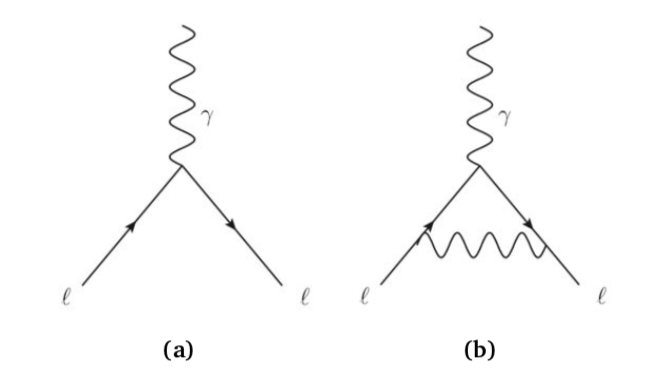
\includegraphics[scale=0.7]{Figures/dirac_g}
\decoRule
\caption{Feynman diagrams of (a) the Dirac term and (b) the Schwinger, leading-order, QED contribution $a_{l}$.}
\label{fig:dirac_g}
\end{figure}

\begin{equation}
a_{l} = \frac{g_{l}-2}{2}.
\end{equation}
Although the majority of the anomaly originates from QED processes, there are smaller contributions from electroweak and hadronic processes which will be discussed later in section~\ref{sec:sm_amu}.
%----------------------------------------------------------------------------------------

\section{The anomalous magnetic moment of the muon}
\label{sec:amm}

The current theoretical predictions and experimental measurements of the electron anomaly $a_{e}$ are the most precisely determined quantities to date \cite{Reference8}. The sensitivity of lepton anomalous magnetic moments to new physics at higher energy scales ($\Lambda$) is proportional to  $m_{l}^2/\Lambda^2$. As the muon is approximately 200 times heavier than the electron, this results in the muon being more sensitive to effects from heavy particles compared to the electron despite the fact that $e_e$ is determined with a precision approximately 2,000 times better than $a_\mu$. Therefore in principle the tau lepton would make the best choice for probing the BSM physics. However the tau lifetime is far too short to be able to carry out a precise enough measurement. The relatively long lifetime and large mass of the muon makes $a_{\mu}$ the best candidate for BSM physics searches, and several precision $a_{\mu}$ measurements have been made. 

The most precise of these $a_{\mu}$ measurements was achieved by the Brookhaven National Laboratory (BNL) muon g-2 experiment, which ran between 1997 and 2001 and measured $a_{\mu}$ to a precision of 540 ppb \cite{Reference13}, a technique which was first adopted at CERN in 1958, as discussed in the next chapter. This experiment utilised a large magnetic storage ring in which orbiting muons were stored. The precession of the muons spin vector due to the muon magnetic moment in the presence of a magnetic field was measured. This gave a surprising result with the measurement deviating from the SM prediction by 3.3$\sigma$ to 3.6$\sigma$.

The Fermilab g-2 experiment will investigate this deviation further. Should the comparison of both theory and experiment yield an agreement, this would prove another success for the SM. However, if a discrepancy exists between the SM prediction $a_{\mu}^{SM}$ and the experimental measurement $a_{\mu}^{exp}$, this would indicate the existence of BSM physics.

\subsection{The history of muon g-2 measurements}

An experimental value of $a_{\mu}$ was not directly measured until the CERN I experiment in 1958. There were three experiments at CERN and another at Brookhaven National Laboratory prior to the Fermilab g-2 experiment. All these experiments relied on the same methodology of determining an $a_{\mu}$ value from $\omega_{a}$, which is determined from the measurement of the frequency at which the spin vector precesses relative to the momentum vector.

In 1957 parity violation was discovered and it was found that highly polarized muon beams could be produced. This will be explained in chapter 3. It was also discovered that the angular distribution of the highest momentum decay electrons would indicate the spin direction of the muon as a function of time \cite{Reference9}. 
Therefore the use of polarised muons from parity violating weak decays allowed the decay angle to be determined. These realisations enabled the basic principles for all subsequent muon g-2 experiments. 

\subsection{CERN I (1958-1962)}
The CERN I experiment located in the experimental hall of the CERN Synchro-Cyclotron became the first experiment to determine a value of the muon anomalous magnetic moment $a_{\mu}$. A 6m 1.5 T bending magnet was constructed containing a uniform field between two rectangular pole pieces as shown in figure 2.2. This enabled muons to achieve up to 2000 turns within the muon storage time period of 2$\mu$s - 8$\mu$s. The muons were injected inside the magnet and directed towards an absorber material inside the magnetic field. Upon collision this caused the muons to lose energy and change direction, leading to a circular orbit. This resulted in the storage of the muons inside the magnetic field region. A transverse magnetic field gradient was used to ensure the muons did not subsequently hit the absorber material again on their subsequent turns and to guide the muons horizontally from one side of the magnet to the other.
At the opposite end of the magnet, a large magnetic gradient was used to eject the muons from the magnet and aim them at an absorber, causing the muons to stop and decay into positrons. The spin directions of the incident muons were measured by recording the decay positron in forward and backward counters. Finally the storage time was determined by counters at either end of the magnet\cite{Reference10}. 

This experiment determined an $a_{\mu}$ value of \cite{Reference11} \cite{Reference12}
\begin{equation}
a_{\mu} = 116500000(500000){\times}10^{-11}
\end{equation}

\begin{figure}[th]
\centering
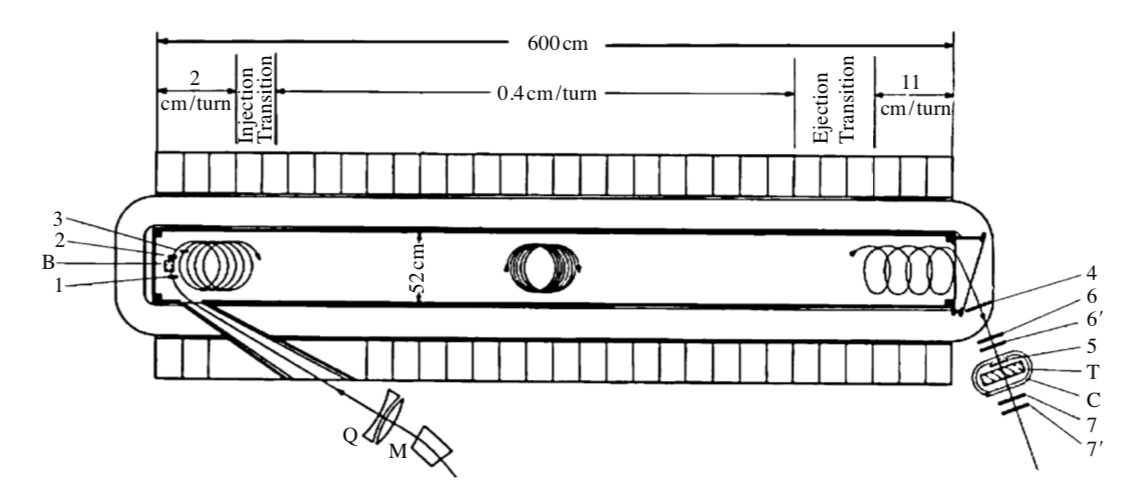
\includegraphics[scale=0.7]{Figures/cern1}
\decoRule
\caption{ A diagram showing the 6m bending magnet used for storing muons. The muons enter through a bending magnet (M) and the quadrupole pair (Q) enable the correct cyclotron radius. The muons are directed to a target (B), follow a circular orbit and drift towards the opposite end of the magnet where they are ejected from the magnetic field. Here they are stopped by an absorber and decay into electrons. The storage time of the muon in the magnetic field was recorded by coincidences in counters 123 at the input, and at the output with counters 466' 57' \cite{Reference10}.}
\label{fig:cern1}
\end{figure}

\subsection{CERN II (1962-1968)}

By now it had been acknowledged that the optimal way to test QED at short distances was by measuring the muon anomalous magnetic moment. A need for higher precision experiments was required to test QED further. To achieve this, the experiment needed to store a larger number of muons for an increased amount of time in order to observe more muon g-2 cycles. The new CERN proton synchrotron (PS) was ideal as it could supply higher energy muons of order GeV and therefore the muons produced would possess relativistically dilated lifetimes. This allowed for a larger number of cycles around the ring, with the g-2 precession frequency unaffected by the time dilation. This experiment became the first experiment to measure $a_{\mu}$ directly and also the first muon g-2 experiment to utilise a weak focusing magnetic field storage ring.

The injection of 10.5 GeV protons onto a pion production target situated inside a 5 m diameter storage ring volume lead to an increased number of muons available for the experiment. A diagram of the CERN II setup is shown in figure 2.3. The pions subsequently decayed in flight to produce muons. The stored muons were mainly from forward pion decays that had lost a small amount of energy and as such did not strike the production target in further orbits of the ring.
Muons required a momentum of 1.28 GeV/c in order to stay in orbit. This corresponds to a gamma factor $\gamma$ = 12 giving a relativistically dilated lifetime of 27 $\mu{s}$. These muons subsequently decayed to electrons which curled inwards towards the ring due to their lower energy and were recorded by counting detectors at a rate which was modulated at the $\omega_{a}$ frequency. This experiment improved the accuracy of $a_{\mu}$ by a factor of 15. Leading to an $a_{\mu}$ value of \cite{Reference10}\cite{Reference12}.

\begin{equation}
a_{\mu} = 116616000(31000){\times}10^{-11}
\end{equation}

\begin{figure}[th]
\centering
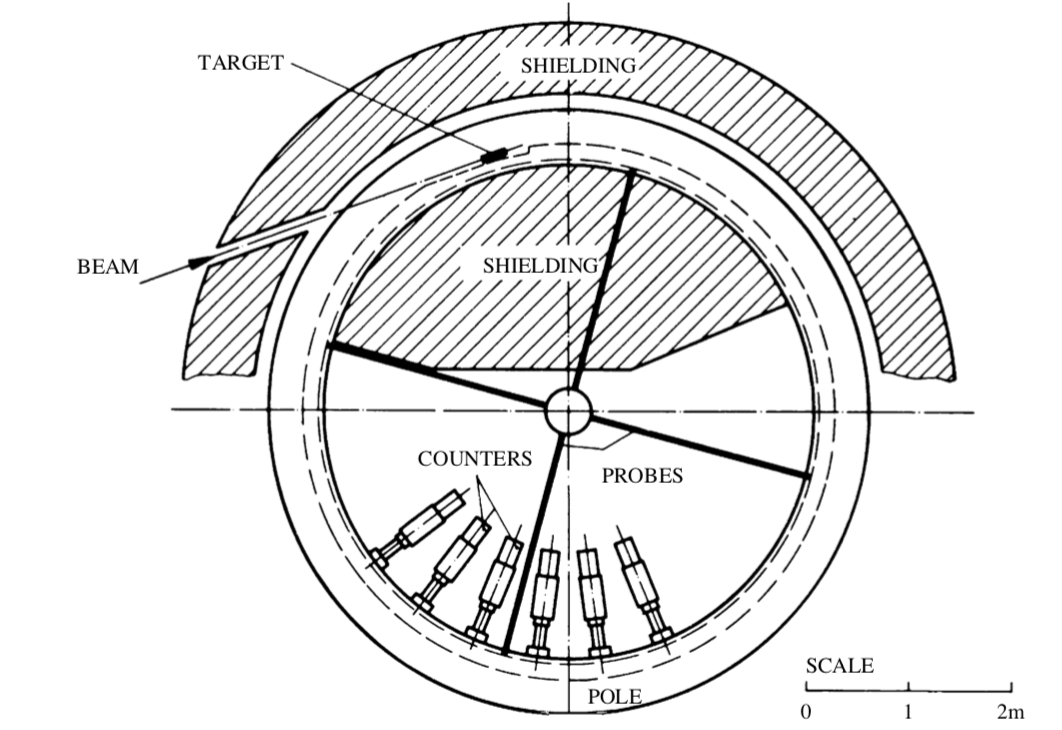
\includegraphics[scale=0.7]{Figures/cern2}
\decoRule
\caption{A diagram of the first muon storage ring used in the CERN II experiment. Protons were injected directly into the storage ring, with pions produced at the target which decayed to muons. The muons with a momentum of 1.28 GeV/c were stored and orbited the ring. These muons subsequently decayed to electrons and were recorded by the counting detectors. The electron hit rate was used to obtain $a_{\mu}$ \cite{Reference10}.}
\label{fig:cern2}
\end{figure}

\subsection{CERN III (1969-1976)}

The CERN III experiment subsequently improved on the muon storage ring method with a new 14 m diameter storage ring installed in the CERN Super Proton Synchrotron (SPS). The setup of CERN III is shown in figure 2.4. This experiment introduced the use of the muon "magic" momentum. It was discovered that if the selected muons had a momentum of 3.094 GeV/c this would cancel out the effects of the radial electric field. This will be discussed in section 3.6. Thus vertical focusing can be provided by electrostatic quadrupoles rather than magnetic gradient focusing and so a very uniform magnetic field can be utilised. This enabled a more precise determination of the magnetic field which was advantageous due to magnetic field variations being a large source of systematic error in the CERN II experiment. The magic momentum gives at a relativistic factor of $\gamma$ = 29.3 and a time dilated lifetime of 64 $\mu{s}$, meaning that the muons could traverse the storage ring an increased number of times. The experiment also utilised pion injection rather than proton injection which reduced the background and increased the beam intensity. These improvements led to an uncertainty on $a_{\mu}$ of 8ppm giving a value of \cite{Reference10}\cite{Reference12}

\begin{equation}
a_{\mu} = 116 592 300(800){\times}10^{-11}
\end{equation}

\begin{figure}[th]
\centering
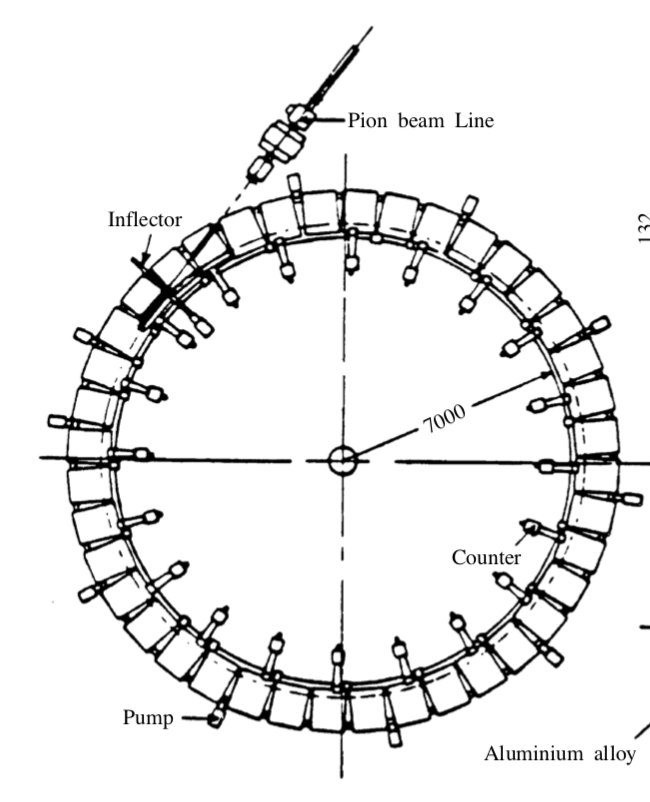
\includegraphics[scale=0.7]{Figures/cern3}
\decoRule
\caption{A diagram of the CERN III experiment which was the second experiment to use a muon storage ring. This ring consisted of 40 contiguous magnet blocks, with decay electrons being detected by 20 counters placed around the ring \cite{Reference10}.}
\label{fig:cern3}
\end{figure}

\subsection{The E821 experiment at the Brookhaven National Laboratory (1984-2003)}

The Brookhaven National Laboratory's E821 experiment carried out the most precise measurement of the muon anomalous magnetic moment to date with the aim of improving the accuracy of the measurement by a factor of 20 to 350 ppb. This meant that a 400 fold increase in statistics would be required. The experiment repeated the methodology used previously at the CERN experiments with a newly designed storage ring, shown in figure 2.5. This could be achieved by use of the Brookhaven Alternating Gradient Synchrotron \cite{Reference10} which provided the required higher intensity beam. Another improvement from the previous experiment was the injection of muons into the storage ring rather than pions. Muon injection meant data at earlier times after injection could be used for analysis. Due to the exponential decay in the number of muons, detectors were able to record hits at earlier times, leading to an increase in statistics. Improvements to the magnetic field measurements were carried out through the use of a trolley which transported 17 nuclear magnetic resonance (NMR) probes around the ring along with 360 stationary NMR probes \cite{Reference10}. 
The experiment ultimately achieved an uncertainty on $a_{\mu}$ of 540 ppb, giving a value of \cite{Reference13}\cite{Reference14}

\begin{equation}
a_{\mu} = 116 592 082(54){\times}10^{-11}
\end{equation}

The experimental value was revealed to differ from the theoretical prediction by 3.3$\sigma$ - 3.6$\sigma$ depending on which theory model is applied. figure 2.6 shows the experimental precision achieved on all the previous $a_{\mu}$ measurements along with the goal precision for the Fermilab E989 experiment of 140 ppb. 

\begin{figure}[th]
\centering
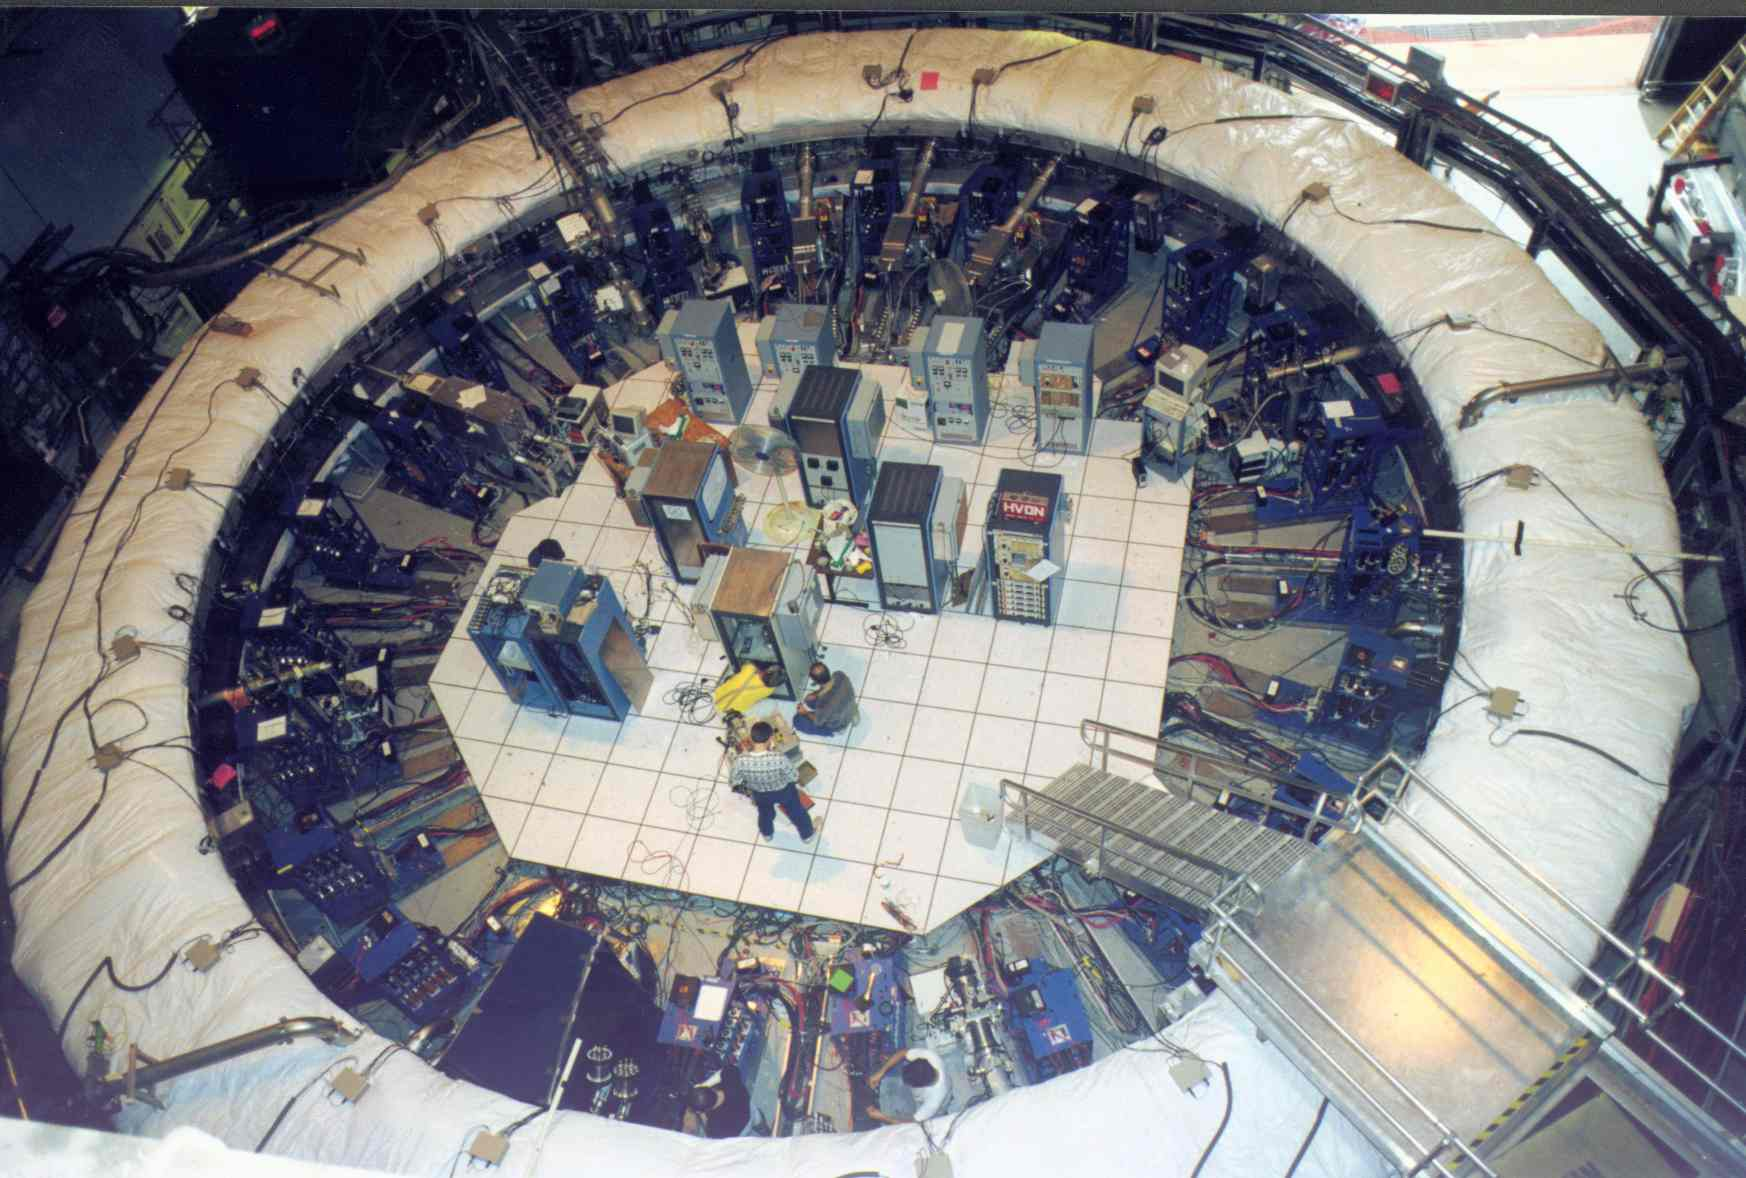
\includegraphics[scale=0.7]{Figures/bnl}
\decoRule
\caption{The BNL experiment magnetic storage ring.}
\label{fig:bnl}
\end{figure}

\begin{figure}[th]
\centering
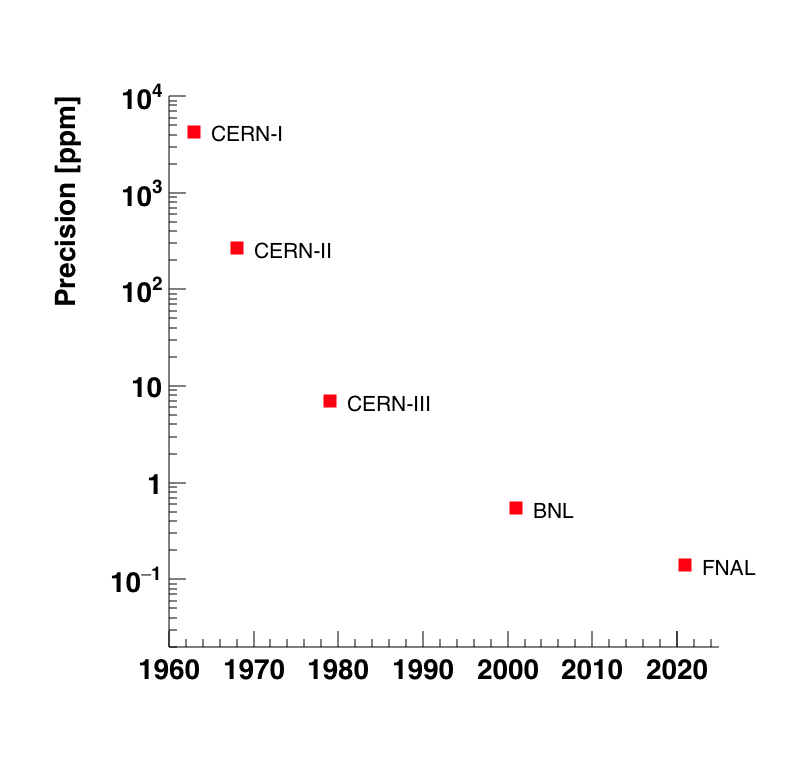
\includegraphics[scale=0.5]{Figures/gm2_precision_vs_time.png}
\decoRule
\caption{A plot displaying the precision achieved by $a_{\mu}$ measurements for all previous experiments and the target $a_{\mu}$ precision for the current Fermilab experiment.}
\label{fig:gm2_precision_vs_time.png}
\end{figure}

\section{Standard model value of $a_{\mu}$}
\label{sec:sm_amu}

The high precision to which $a_{\mu}$ has been and is intended to be measured demands corresponding precision in the SM theoretical prediction. The comparison between the experimental and theory provides a test of the completeness of the SM. In the SM, contributions to $a_{\mu}$ involve parts from QED, the strong interaction (Had) and the Electroweak (EW) interaction.

\begin{equation}
a_{\mu}^{SM}=a_{\mu}^{QED} + a_{\mu}^{Had} + a_{\mu}^{EW}.
\end{equation}
Each of these contributions will be discussed below, with the contribution to $a_{\mu}^{SM}$ and its uncertainty quoted for each part. 

\subsection{QED contributions to $a_{\mu}$}

The QED contributions dominate the value of $a_{\mu}^{SM}$ at over 99$\%$, but these interactions are very precisely predicted. 
The QED contributions to $a_{\mu}$ consists of all virtual photon and lepton \cite{Reference15} loops. With the leading order contribution consisting of only one contribution ${\alpha}/2{\pi}$, which was first calculated by Schwinger. The Feynman diagram is shown in figure 2.7a. The next to leading order contributions (NLO) consists of nine two loop processes, one of which is shown in figure 2.7b. The QED contributions have been calculated up to and including the five loop interactions. This accuracy was recently achieved by Kinoshita et al. and required the calculation of 12672 Feynman diagrams \cite{Reference16}\cite{Reference17}. Several of which are shown in figure 2.8. Therefore even though QED has the largest contribution to $a_{\mu}^{SM}$, it has the smallest uncertainty ${\delta}a_{\mu}^{SM}$.

The SM theoretical value for the QED contribution to the anomalous magnetic moment is given by

\begin{equation}
a_{\mu}^{QED} = 116 584 718.97(0.07){\times}10^{-11}
\end{equation}

\begin{figure}[th]
\centering
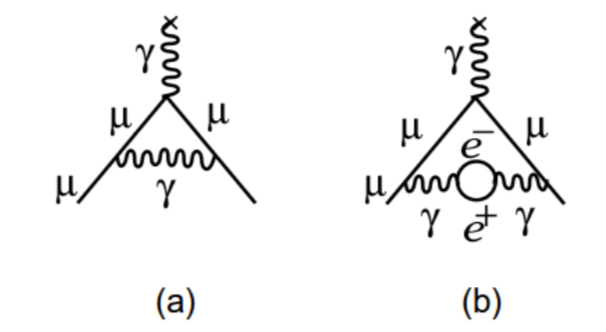
\includegraphics[scale=0.6]{Figures/QED_LO_NLO}
\decoRule
\caption{(a) Leading order and (b) next to leading order Feynman diagrams of QED contributions to $a_{\mu}$}
\label{fig:QED_NO_NLO}
\end{figure}

\begin{figure}[th]
\centering
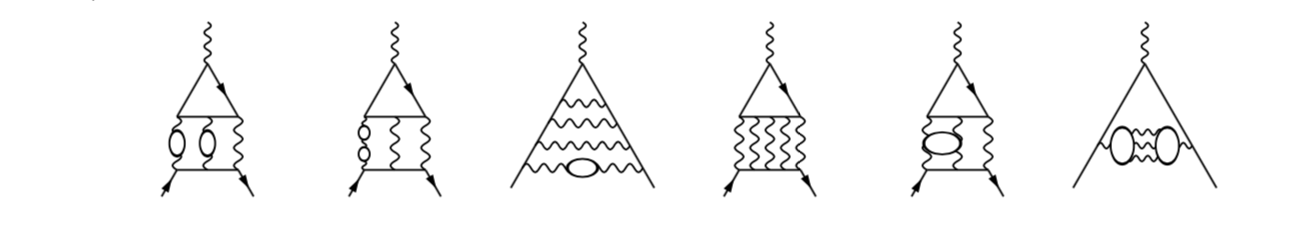
\includegraphics[scale=0.6]{Figures/QED5loop}
\decoRule
\caption{Feynman diagrams for a number of typical five-loop QED  contributions}
\label{fig:QED5loop}
\end{figure}

\subsection{Electroweak contributions to $a_{\mu}$}

The electroweak interactions contribute the lowest amount to $a_{\mu}^{SM}$, which consist of loops from $W^{\pm}$ and Z bosons along with the Higgs boson. The large masses of the W and Z bosons lead to a reduction of their effect on $a_{\mu}^{EW}$ and therefore the electroweak contribution is small. Electroweak contributions to the anomalous magnetic moment are shown in figure 2.9. These interactions are well known to the two-loop accuracy where the LO contributions from the W and Z bosons contribute largely to the value \cite{Reference18}\cite{Reference19}.

\begin{figure}[th]
\centering
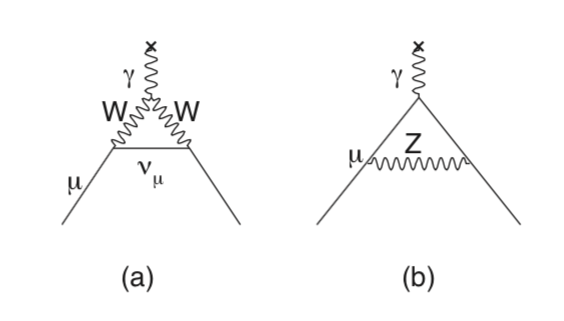
\includegraphics[scale=0.7]{Figures/weakContribution}
\decoRule
\caption{Electroweak contributions to the anomalous magnetic moment. (a) Illustrates the largest contribution to $a_{\mu}^{EW}$. It involves the conversion of the muon to an appropriately charged W boson, with the emission and subsequent recapture of a muon neutrino. (b) The LO Electroweak interaction. It is identical to the Schwinger term, except the photon has been substituted for a Z or Higgs boson}
\label{fig:weakContribution}
\end{figure}

The SM theoretical value for the Electroweak contribution to the anomalous magnetic moment is given by

\begin{equation}
a_{\mu}^{EW} = 153.6(1.0){\times}10^{-11}
\end{equation}

\subsection{Hadronic contributions to $a_{\mu}$}

The Hadronic effects contribute the largest uncertainty on the anomaly $a_{\mu}$. These effects originate from virtual quark and gluon loops interactions that can be divided into two subcategories: the hadronic vacuum polarisation (HVP) and the hadronic light-by-light (HLbL).

\begin{equation}
a_{\mu}^{had} = a_{\mu}^{HVP} + a_{\mu}^{HLbL}
\end{equation}

The Hadronic contributions, unlike the QED and Electroweak contributions, cannot be determined perturbatively \cite{Reference20}. This is because the energy scale is of the order $m_{\mu}c^2$ for virtual hadrons, which lies below the perturbative region of QCD. Instead the HVP calculation relies on experimental data. In this case data from ${e^+}{e^-}$ experiments can be used to make this calculation. This is because the HVP contribution to $a_{\mu}$ can be related via the dispersion relation to the cross section for ${e^+}{e^-}$ annihilation into hadrons. Thus the measured cross sections of ${e^+}{e^-}$ annihilation into hadrons is used to make a HVP calculation \cite{Reference21}. An example of a Feynman diagram for HVP is shown in figure 2.10. The HVP contribution determined from the dispersion relation is given by

\begin{equation}
a_{\mu}^{had;LO} = \Big(\frac{\alpha{m}_{\mu}}{3\pi}\Big)^{2}\int^{\infty}_{m^{2}_{\pi}} \frac{ds}{s^2}K(s)R(s), 
\end{equation}

\begin{equation}
\text{where } R = \frac{\sigma_{tot}(e^{+}e^{-} \rightarrow hadrons)}{\sigma(e^{+}e^{-} \rightarrow \mu^{+}\mu^{-})},
\end{equation}

where K(s) is a kinematic factor with a range of 0 at s = $\infty$ to 0.4 for s = $m^{2}_{\pi}$ \cite{DispersionRel}.
Due to $s^2$, the calculation of $a_{\mu}^{had;LO}$ is dominated by the R(s) values at low energies. And for the required precision, data of up to 2 GeV is useful \cite{Reference29}. Cross-section data from a range of experiments including KLOE, BaBar, BELLE, VEPP and BES have been combined in order to determine the HVP contribution \cite{Reference22}.

\begin{figure}[th]
\centering
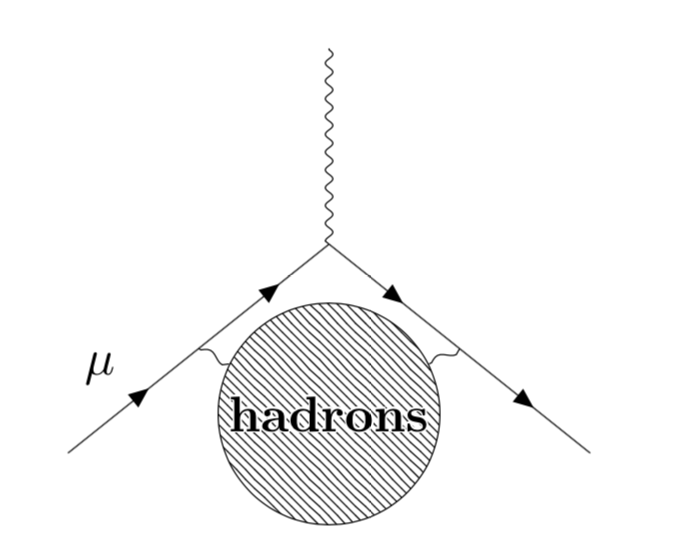
\includegraphics[scale=0.7]{Figures/HadHVP}
\decoRule
\caption{The Feynman diagram of the LO hadronic vacuum polarisation contribution to $a_{\mu}$}
\label{fig:HadHVP}
\end{figure}

The Hadronic LbL contributions are calculated by combining the results of various model dependent approaches \cite{Reference23}. The LO Hlbl Feynman diagram is shown in figure 2.11. To date the most accurate estimate of these contributions was made by an international group of theorists known as the "Glasgow" consensus \cite{Reference24}. However the determined uncertainty remains relatively large. Although HLbL scattering contributions only account to a tiny percentage of the total value of $a_{\mu}^{SM}$, they contribute approximately 53$\%$ to the uncertainty value \cite{Reference25}.

\begin{figure}[th]
\centering
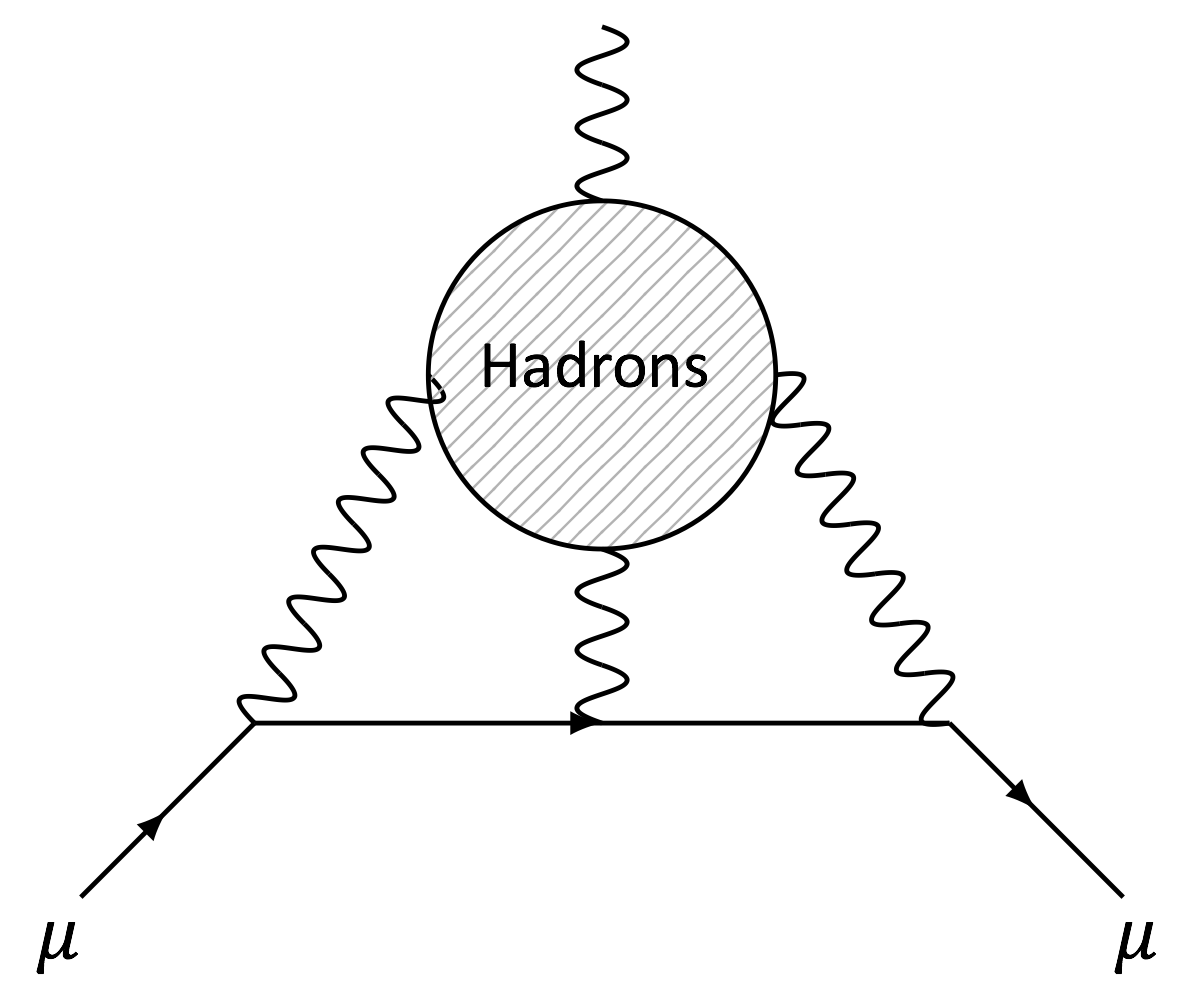
\includegraphics[scale=0.4]{Figures/hadroniclbl.png}
\decoRule
\caption{Feynman diagram showing  LO Hadronic light-by-light process}
\label{fig:hadroniclbl}
\end{figure}

The SM theoretical value for the Hadronic contributions to the anomalous magnetic moment is given by

\begin{equation}
a_{\mu}^{HVP} = 6933(25){\times}10^{-11}
\end{equation}

\begin{equation}
a_{\mu}^{HLbL} = 980(26){\times}10^{-11}.
\end{equation}

\subsection{Value and uncertainty of $a_{\mu}^{SM}$}

The SM contributions can be summed together to give an overall calculation of the SM value $a_{\mu}^{SM}$ and its uncertainty ${\delta}a_{\mu}^{SM}$ \cite{Reference26}\cite{Reference27}. The individual contributions to $a_{\mu}^{SM}$ are shown in Table 2.1.

\begin{table}[h!]
\begin{center}
 \begin{tabular}{||c | m{5cm}||} 
 \hline
 Contribution & Result $(10^{-11})$ \\ [0.5ex] 
 \hline\hline
 QED (leptons) & 116 584 718.97 $\pm$ 0.07 \\ 
 \hline
 HVP & 6933 $\pm$ 25 \\
 \hline
 Hlbl & 980 $\pm$ 26 \\
 \hline
 EW & 153.6 $\pm$ 1.0 \\
 \hline
 Total SM & 116591820.4 $\pm$ 35.6 \\ [1ex] 
 \hline
\end{tabular}
\caption{Table of all the contributions to $a_{\mu}^{SM}$}
\label{table:1}
\end{center}
\end{table}
\noindent

The SM value of $a_{\mu}^{SM}$ is calculated to be

\begin{equation}
a_{\mu}^{SM} = 116591820.4(35.6){\times}10^{-11}
\end{equation}

As mentioned previously the current highest precision experimental measurement of $a_{\mu}$ was carried out at BNL in 2001 \cite{Reference27}\cite{Reference28} giving

\begin{equation}
a_{\mu}^{Exp} = 116592091(54)(33){\times}10^{-11}
\end{equation}

Where the value in the first bracket is the statistical uncertainty and the value in the second bracket is the systematic uncertainty. The difference between the experimental and theoretically calculated $a_{\mu}$ is

\begin{equation}
a_{\mu}^{Exp} - a_{\mu}^{SM} = 270.6{\pm}72.6{\times}10^{-11}
\end{equation}

The SM theoretical value is currently 3.3-3.6$\sigma$ \cite{Reference29} below the most recent experimental measurement. If this difference observed is not a statistical fluctuation, this would indicate the presence of as yet to be discovered physics processes that affect the value of $a_{\mu}$.

To investigate this discrepancy a new experiment, the Fermilab E989 muon g-2 experiment has been designed to improve on the accuracy of the BNL experiment by a factor of four. If the value of $a_{\mu}$ is unchanged after this experiment, the improved statistics will mean a 5$\sigma$ or more deviation from the SM as shown in figure 2.12. Efforts to further improve the SM theory are simultaneously taking place. 
The value of the anomaly will be an important precision frontier measurement which will help to guide the understanding of any BSM physics discovered.

\begin{figure}[th]
\centering
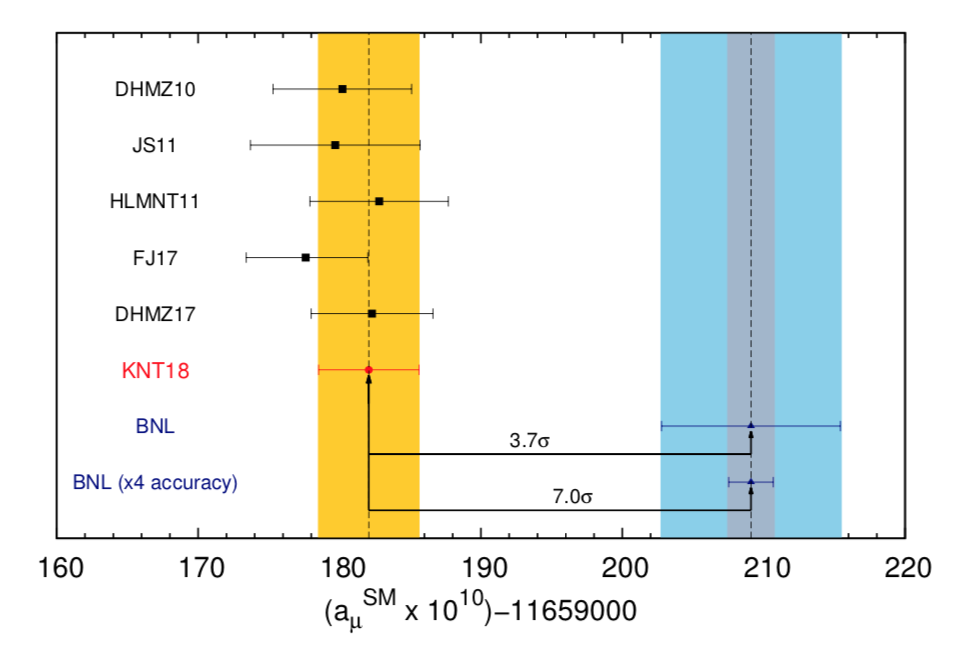
\includegraphics[scale=0.7]{Figures/SManomalousMagMom}
\decoRule
\caption{A comparison of recent evaluations of $a_{\mu}^{SM}$.}
\label{fig:SManomalousMagMom}
\end{figure}

%----------------------------------------------------------------------------------------

\section{Possible new physics contributions to $a_{\mu}$}

A possible explanation for the discrepancy between the experimental and theoretical prediction of $a_{\mu}$ come from BSM physics contributions. For most BSM theories the contribution to $a_{\mu}$ decreases as the mass scale of the BSM physics increases. Therefore the deviation in the value observed by BNL points to new physics existing in an energy scale of up to a TeV.

The muon anomalous magnetic moment provides a unique probe into BSM physics due to its unique properties. Any possible BSM contributions must be CP and flavour conserving and flip the chirality of the muon. These properties are in contrast to a lot of other low energy precision and high energy collider experiments.

There are a variety of BSM models that could explain the anomaly. These include Supersymmetry (SUSY), the existence of further electroweak bosons like W' or Z' and additional Higgs models \cite{Reference1}.
One of these SUSY theories explains that the anomaly can be described through conversions to supersymmetric particles such as the sneutrino-chargino and the smuon-neutralino. The Feynman diagrams are shown in figure 2.13. This is where the muon will briefly convert into either of these supersymmetric pairs before returning to a muon \cite{Reference30}. In this SUSY theory, the amount it contributes to the value of $a_\mu$ is dependant on the sign of the $\mu$ parameter, the SUSY mass scale and and the value of \mathrm{tan}$\beta$ \cite{Reference30}.

\begin{equation}
|a_{\mu}^{SUSY}| \approx (sgn\mu) 130\times10^{-11} tan\beta \Big(\frac{100GeV}{\tilde{m}}\Big)^2.
\end{equation}
\noindent
With \mathrm{tan}$\beta$ being set to approximately 50, the anomaly currently observed can be explained by putting the muon mass scale at ${\tilde{m}} \approx 500GeV/c$ \cite{Reference31}\cite{Reference32}. 

\begin{figure}[th]
\centering
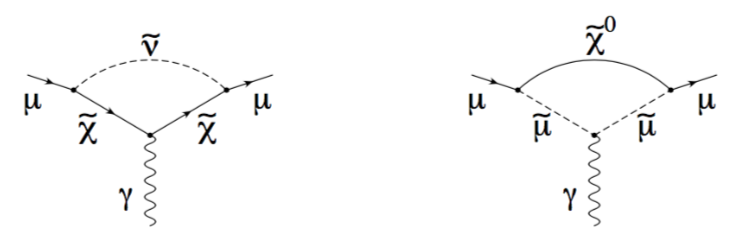
\includegraphics[scale=0.7]{Figures/SUSY}
\decoRule
\caption{Feynman diagrams of two SUSY interactions which would contribute to the anomalous magnetic moment. The left diagram, shows the muon briefly converting into a chargino $\tilde{\chi}$ and a sneutrino $\tilde{\nu}$. The right showing the muon briefly converting to a smuon $\tilde{\mu}$ and a neutralino $\tilde{\chi}^0$.}
\label{fig:SUSY}
\end{figure}

The measurement at Fermilab will provide further restrictions on viable BSM models. If such new physics is discovered elsewhere, for instance at the LHC, then $a_{\mu}$ will play an important role in determining the interpretation of those discoveries. If no new discoveries are found elsewhere, then it represents one of the few methods to probe BSM physics. In either case, it will play a major role in the search to understand BSM physics at the TeV scale.



%----------------------------------------------------------------------------------------


